\documentclass{sigchi}

\toappear{CS3301: Component Technology Practical 1: Middleware}

\pagenumbering{arabic}

\usepackage{balance} 
\usepackage{graphics}
\usepackage{times}
\usepackage{url}
\usepackage{amsmath}
\newcommand{\BigO}[1]{\ensuremath{\operatorname{O}\bigl(#1\bigr)}}

\makeatletter
\def\url@leostyle{%
  \@ifundefined{selectfont}{\def\UrlFont{\sf}}{\def\UrlFont{\small\bf\ttfamily}}}
\makeatother
\urlstyle{leo}

\def\pprw{8.5in}
\def\pprh{11in}
\special{papersize=\pprw,\pprh}
\setlength{\paperwidth}{\pprw}
\setlength{\paperheight}{\pprh}
\setlength{\pdfpagewidth}{\pprw}
\setlength{\pdfpageheight}{\pprh}

\usepackage[pdftex]{hyperref}
\hypersetup{
pdftitle={SIGCHI Conference Proceedings Format},
pdfauthor={LaTeX},
pdfkeywords={SIGCHI, proceedings, archival format},
bookmarksnumbered,
pdfstartview={FitH},
colorlinks,
citecolor=black,
filecolor=black,
linkcolor=black,
urlcolor=black,
breaklinks=true,
}
\providecommand*{\lstnumberautorefname}{line} 
\newcommand\tabhead[1]{\small\textbf{#1}}

\usepackage{color}
\usepackage{upquote}
\usepackage{listings}
\lstset{ %
upquote=true
basicstyle=\footnotesize,       % the size of the fonts that are used for the code
numbers=left,                   % where to put the line-numbers
numberstyle=\footnotesize,      % the size of the fonts that are used for the line-numbers
stepnumber=1,                   % the step between two line-numbers. If it is 1 each line will be numbered
numbersep=5pt,                  % how far the line-numbers are from the code
backgroundcolor=\color{white},  % choose the background color. You must add \usepackage{color}
showspaces=false,               % show spaces adding particular underscores
showstringspaces=false,         % underline spaces within strings
showtabs=false,                 % show tabs within strings adding particular underscores
frame=single,           % adds a frame around the code
tabsize=2,          % sets default tabsize to 2 spaces
captionpos=b,           % sets the caption-position to bottom
breaklines=true,        % sets automatic line breaking
breakatwhitespace=false,    % sets if automatic breaks should only happen at whitespace
escapeinside={\%*}{*)}          % if you want to add a comment within your code
}
\renewcommand\lstlistingname{Code Fragment}

\usepackage[english]{babel}
\usepackage[autostyle]{csquotes}

\begin{document}

\title{Component Technology - Middleware}

\numberofauthors{2}
\author{
  \alignauthor 110011264\\
    \affaddr{School of Computer Science}\\
    \affaddr{University of St Andrews}\\
  \alignauthor 110002255\\
    \affaddr{School of Computer Science}\\
    \affaddr{University of St Andrews}\\
}

\maketitle

\begin{abstract}
Abstract
\end{abstract}

\section{REPORT}

\subsection{Planning}

Initially, the team implemented a simple server. The server receives heartbeats, in the form of POST request, from the producers. Each heartbeat consisted of an unique identifier of the mobile phone device and its current location. The sender advertises itself as a producer to the server. When a consumer asks the server for sensor data from that particular producer, the server will send a request to the producer, and then pass on the results back to the producer. However, this approach requires the producers listening on some ports to handle data requests from the server. As a result, the consumer will spend significant time waiting for the server to retrieve data from the producer. The solution will create too much overhead on the server side, and it is unlikely that the server can deal with increasing consumer requests.

Later on, the team arrived to a more elegant solution. On each heartbeat, the producer sends sensor data to the server. The server caches the data, and flushes them to a persistent database on occasion. Now, when a consumer requests sensor data from a particular producer, the server can respond quickly, since the sensor data are cached. A more detailed description of the overall setup is explained in the next

\subsection{Instructions}

See \enquote{README.md} in the project directory for directions on how to run the servers, producers, and consumers.

\subsection{Design}

\subsubsection{System components}

The final system architecture at the time of our submission consists of:

\begin{itemize}
  \item 1 Load balancer
  \item N Workers
  \item X Producers
  \item Y Consumers
\end{itemize}

A load balancer is the primary component of the system. It manages every other system component and balances the server load. A worker is a separate unit that is responsible for data retrieval and stroage. A producer generates sensor data, and a consumer requests those data. An example of a producer would be a mobile phone, and an example of a consumer would be a web service that uses location data to recommend music to its users.

\subsubsection{Load balancer and workers}

The load balancer is the entry point of the entire system. It is initialised to be listening on a specified port. It supports a number of RESTful API calls that allows other entities to interact with its system componenets, such as a worker. The worker is initialised with the IP address and the port number of the load balancer, so that it can register itself as a worker for the load balancer via with the $/balancer/port$ API call. The load balancer processes the registration request, and stores the worker's IP address in memory. The load balancer keeps track of every worker, and will distribute the sever load equally, using the round robin method. Every worker must go through the above registration process in order to let itself known to the load balancer, whom will redirect producers and consumers to the worker. The worker also listens on a specified port, for handling heartbeats (described below) and sensor data requests.

\subsubsection{Load balancer and producers}

The producers need to go through the balancer in order to get a worker assigned to them. The balancer uses the list of online workers to assign a worker. A round robin approach is used to ensure that the load is distribute evenly to all workers and is almost the same at every given time for every worker.
An API call /register/<int:id> is made by the producer to the balancer with its ID. The balancer keeps track of the relationship between producers and workers which is used when the consumer requests are handled. When a worker is found, the producer gets redirected to it and the communication between the producer and balancer is over.

A typical use case:
A producer is started by providing a balancer address and producer ID. The finds a worker for the producer or returns a message that no workers are available. If a worker is available the corresponding address is returned. All errors regarding connection loss or interruption are handled.

\subsubsection{Workers and producers: heartbeats}

After a producer receives its assigned worker address it starts sending heartbeats (periodic messages). They contain the following information:

\vspace*{\baselineskip}
\begin{lstlisting}[caption={Heartbeat format}, mathescape, upquote=true]
received_heartbeat = {
  'id': id
  'location': location
  'data': data
}

new_heartbeat = {
  'id': int(request.json['id']),
  'location': request.json['location'],
  'ip_address': request.remote_addr,
  'timestamp': datetime.utcnow(),
  'data': request.json['data']
}
\end{lstlisting}

DATABSE STUFF HERE
If the worker goes offline / crashes the producer can try to reconnect a specified number of times. It does that through the balancer so if more workers are available it immediately gets given a worker or the moment a worker becomes available. The number of retries can be specified by the user and it can be indefinite, meaning the producer can always be looking for a connection.

A typical use case:
A producer receives a worker address from the balancer and uses it to start making hearbeats to the worker, providing data and information. If the worker happens to go down, a retry mechanism triggers and the producers tries to re-register with the balancer. If workers are available the producer gets a new worker and continues heartbeats. All errors regarding connection loss or interruption are handeled.

On each heartbeat POST request, the worker extracts the \enquote{id}, \enquote{location}, and \enquote{data}. In addition, the worker takes note of the remote IP address of the request, as well as the current time. The worker puts the information altogether into a \enquote{heartbeat} object (a dictionary in $Python$). The team has designed a data structure called cache, defined in $worker/cache.py$. In essence, the cache stores a mapping (another dictionary) between the producer ID and the its latest \enquote{heartbeat}. The worker will flush the \enquote{heartbeats} to the database every $20$ seconds. The time interval is chosen for demonstration purposes, and more tests are needed to find out the optimal time. The worker will also flush the cache to the database when it reaches the size limit. The size is kept to $100$, also for demonstration purposes. When the cache is full and the contained data are added to the database, half of the cache is cleared to allow more data to be added.

\subsubsection{Load balancer and consumers: redirection}

When a consumer requests data it does it through the balancer. As mentioned above the balancer keeps track of the relationship between producers and workers. It redirects the consumer to the appropriate worker to where the data is being stored / received in real time.

A typical use case:
A consumer makes a GET request to the balancer. The balancer checks if the ID of the specified producer is being handled by some of the workers. If so the consumer get redirected to the appropriate worker which will handle the request. All connection errors that might occur that might occur are handeled and do not cause crashes.

\subsubsection{Workers and consumers}

The worker does several things after being contacted by a redirected consumer. First it checks if the requested producer is online and sending that. If yes, then it gets the data from the cache without making queries to the database. In case that the producer is unreachable and there is no current data in the cache a call to the database is made. This greatly reduces the number of database queries while imroving response times.

A typical use case:
A consumer get redirected to a worker. The worker checks if live data for the ID is available in the cache. If not it makes a query to the database. The data is returned to the consumer.


\subsubsection{Why Flask?}
Becuase

\subsubsection{Why RESTful?}

Because

\subsubsection{Why SQLite3?}

Premature optimization is the root of all evil.

\begin{figure}[!h]
\centering
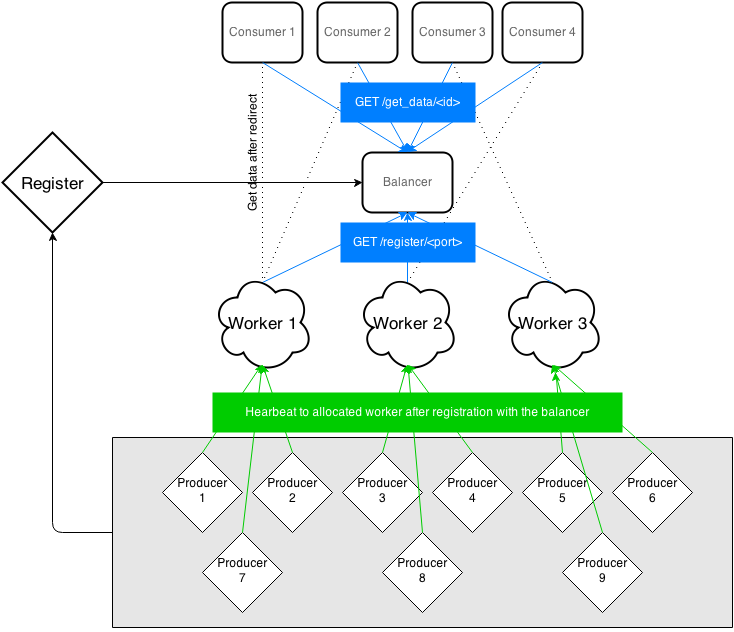
\includegraphics[width=0.9\columnwidth]{img/main}
\caption{The final system architecture}
\label{fig:main}
\end{figure}

\begin{figure}[!h]
\centering
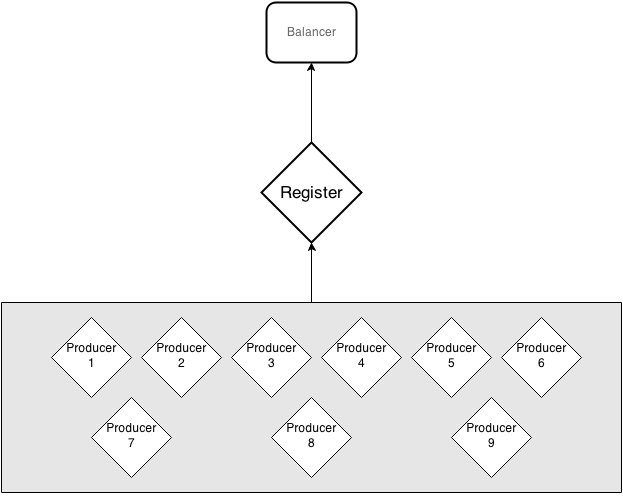
\includegraphics[width=0.9\columnwidth]{img/producer}
\caption{A producer first registers with the balancer and is assigned a worker}
\label{fig:producer}
\end{figure}

\begin{figure}[!h]
\centering
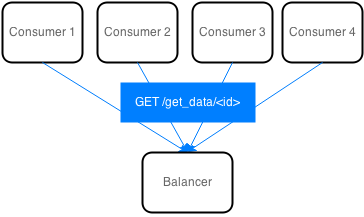
\includegraphics[width=0.9\columnwidth]{img/consumer_req}
\caption{Consumers request data from the load balancer}
\label{fig:consumer_req}
\end{figure}

\begin{figure}[!h]
\centering
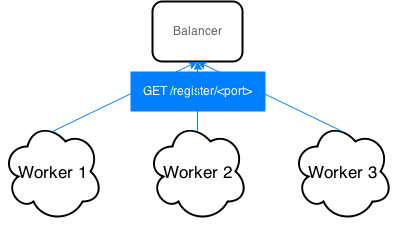
\includegraphics[width=0.9\columnwidth]{img/workerreg}
\caption{Workers need to register with the balancer before they can start accepting work.}
\label{fig:worker}
\end{figure}

\begin{figure}[!h]
\centering
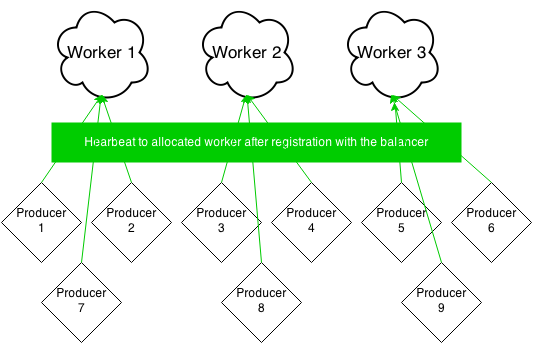
\includegraphics[width=0.9\columnwidth]{img/heartbeat}
\caption{Producers send heartbeats to their assigned workers.}
\label{fig:heartbeat}
\end{figure}

\begin{figure}[!h]
\centering
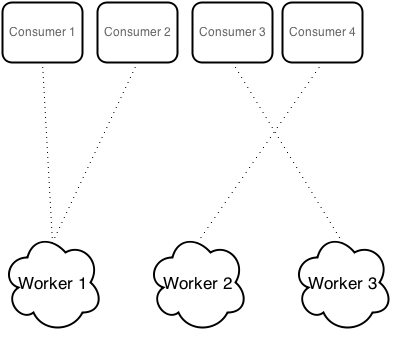
\includegraphics[width=0.9\columnwidth]{img/cons_to_worker}
\caption{Cons to worker}
\label{fig:cons_to_worker}
\end{figure}

\subsection{Evaluation}

\subsection{Testing}

\end{document}
